% Preamble
\documentclass[11pt]{amsart}
\usepackage{mathtools}
\usepackage{amssymb,latexsym}
\usepackage{physics}
\usepackage{listings}
\usepackage{bm}
\usepackage{enumerate}
\usepackage{graphicx}
\usepackage{color}
\usepackage{parskip}
\usepackage{hyperref}
\hypersetup{
    colorlinks=true, % set true if you want colored links
    linktoc=all,     % set to all if you want both sections and subsections 
                     % linked
    linkcolor=blue,  % choose some color if you want links to stand out
}

% Environments
\theoremstyle{definition}
\newtheorem{theorem}{Theorem}
\newtheorem{algorithm}{Algorithm}
\newtheorem{corollary}{Corollary}
\newtheorem*{main}{Main Theorem}
\newtheorem{lemma}{Lemma}[section]
\newtheorem{proposition}{Proposition}
\newtheorem{definition}{Definition}
\newtheorem{example}{Example}
\theoremstyle{remark}
\newtheorem*{notation}{Notation}

% Commands and operators
\newcommand{\ind}{\hspace*{0.5cm}}
\newcommand{\gap}{\hspace*{0.25cm}}
\newcommand*{\Cdot}{\raisebox{-0.25ex}{\scalebox{1.3}{$\cdot$}}}
\newcommand{\vect}[1]{\mathbf{#1}}
\newcommand{\transpose}{\text{T}}
\DeclareMathOperator{\interior}{\textbf{int}}
\DeclareMathOperator{\domain}{\textbf{dom}}
\DeclareMathOperator{\diag}{\textbf{diag}}
\DeclareMathOperator{\sign}{\textbf{sign}}
\DeclareMathOperator{\CG}{\textbf{CG}}
\DeclareMathOperator{\vol}{\textbf{vol}}
\DeclareMathOperator{\CC}{\textbf{CC}}
\DeclareMathOperator{\AC}{\textbf{AC}}
\DeclareMathOperator{\centerr}{\textbf{center}}

\begin{document}
\lstset{language=}
\pagestyle{plain}

\title{Cutting-plane methods for logistic regression and active learning}
\author{David Wu}

\maketitle

% \tableofcontents

\section{Introduction}

    \subsection{Outline.}

    \subsection{Related work.}


\section{Notation and conventions}
    Throughout this paper (unless otherwise stated) we will use the following notation and conventions: 
    \begin{itemize}
        \item We use the notation $Ax \preceq b$ to represent the system of $m$ linear inequalities $a_i^\transpose x \leq b, i = 1, \dots, m$. Therefore, the rows of $A$ and entries of $b$ are given by $a_i$ and $b_i$ respectively, for $i = 1, \dots, m$.
        \item A polyhedron $\mathcal{P}$ is assumed to be defined by linear inequalities $Ax \preceq b$. That is, $\mathcal{P} \coloneqq \{x \;|\; Ax \preceq b\}$.
        \item We make no distinction between a system of linear inequalities $Ax \preceq b$ and the polyhedron $\mathcal{P}$ it defines. The two are synonymous. 
        \item We assume the solution set of $Ax \preceq b$ (and therefore the polyhedron $\mathcal{P}$ it defines) is bounded and, at least initially, non-empty. 
    \end{itemize}  

\section{Cutting-planes and the conceptual cutting-plane algorithm}
    In this section we abstractly introduce the concept of cutting planes and in doing so pave the way to the \emph{conceptual cutting-plane algorithm} (Algorithm \ref{a:conceptual_cp_alg}). This will provide a framework which we can then adapt for the purposes of convex optimization and active learning. Our exposition closely follows S. Boyd and L. Vandenberghe's lecture notes on this topic \cite[Sections 1-3]{BV11}. 


    \subsection{Introduction to cutting-planes}
        Cutting-plane methods address the problem of how to efficiently locate a point in a set $X \subset \mathbb{R}^n$, which we call the \emph{target set}, known to be contained in a polyhedron $\mathcal{P_0}$ defined by linear inequalities $a_i^\transpose x \leq b, i = 1, \dots, m$. 

        \begin{figure}
            \caption{A simple two-dimensional example showing the set-up of the problem.}
        \end{figure}

        The approach of these methods is to iteratively cut away at the polyhedron $\mathcal{P_0}$ until a point in $X$ is found. Formally, starting at the $0$-th iteration, we find a point $x^{(1)}$, which we call the \emph{query point}, in the current (or $0$-th) polyhedron $\mathcal{P}_0$ and check for membership in the target set $X$. If $x$ is a member of $X$ then we are done. If $x^{(1)}$ is not a member of $X$, then we find a halfspace $a_{1}^\transpose x \leq b_{1}$, which we call a \emph{cutting plane}, that seperates, or rather \emph{cuts} $x^{(1)}$ (and other points known not to be in the target set $X$) out of the current iteration's polyhedron $\mathcal{P}_0$. (We allow cuts diretly through the query point $x^{(1)}$, although they are not preferable.) We then conclude the $0$-th iteraton by defining the polyhedron $\mathcal{P}_1$ of the $1$-th iteration to be the union of the $0$-th polyhedron and the $1-th$ cutting plane. In the $1$-th iteration we repeated this process the $1$-th polyhedron $\mathcal{P}_1$. 

        To summarize the discussion so far we present the \emph{conceptual cutting-plane algorithm}:

        \begin{algorithm}[Conceptual cutting-plane algorithm]
        \label{a:conceptual_cp_alg}\mbox{}\\
            \ind \textbf{given} a polyhedron $\mathcal{P}_0 = \{z \:|\: Cz \preceq d\}$ known to contain a target set $X$. \\
            \ind $k \coloneqq 0$. \\
            \ind \textbf{repeat} \\
            \ind\ind Choose a query point $x^{(k+1)} \in \mathcal{P}_k$. \\
            \ind\ind Query the cutting-plane oracle at $x^{(k+1)}$. \\
            \ind\ind If the oracle determines that $x^{(k+1)} \in X$: \\
            \ind\ind\ind\textbf{return} $x^{(k+1)}$. \\
            \ind\ind Else, update $\mathcal{P}_k$ by adding the new cutting-plane: \\ 
            \ind\ind\ind $\mathcal{P}_{k+1} \coloneqq \mathcal{P}_k \cap \{z \:|\: a_{k+1}^\transpose z \leq b_{k+1} \}$. \\
            \ind\ind If $\mathcal{P}_{k+1} = \emptyset$, \textbf{quit}. \\
            \ind\ind $k \coloneqq k+1$.
        \end{algorithm}


    \subsection{Deep cuts and neutral cuts}
        For clearer communication, we will make a distinction between two types of cuts, deep cuts and shallow cuts. A \emph{deep cut with respect to the current iteration's query point $x^{(k+1)}$} is a cut that completely separates that point from the next iteration's polyhedron $\mathcal{P}_{k+1}$ while a \emph{neutral cut with respect to the current iteration's query point $x^{(k+1)}$} is a cut such that that point lies on the boundary of $\mathcal{P}_{k+1}$, that is, a cut that passes directly through the query point $x^{(k+1)}$.

        \begin{figure}
            \caption{A deep cut.}
        \end{figure}

        \begin{figure}
            \caption{A neutral cut.}
        \end{figure}


    \subsection{Adapting the conceptual cutting-plane algorithm for applications}\label{ss:adapt}
        To apply the conceptual cutting-plane algorithm (Algorithm \ref{a:conceptual_cp_alg}) we must specify
        \begin{enumerate}
            \item the target set $X$;
            \item how query points are chosen; 
            \item how cutting-planes are constructed; and 
            \item stopping criterion for the algorithm.
        \end{enumerate}

        Choosing each of these components appropriately will allow us to adapt the conceptual cutting-plane algorithm (Algorithm \ref{a:conceptual_cp_alg}) to convex optimization and active learning. For instance, for convex optimization problems $X$ is typically taken to be some $\epsilon$-suboptimal set while for active learning we take $X$ to be the version space, that is, the set of classification vectors for which the corresponding linear predictors make no mistake on the training data set. Moreover, choosing each of these components also effects the efficiency of the algorithm. 

        For instance, in the applications we  consider we will choose the query point to be an approximation of the current polyhedron's center, for which there are several choices, of varying computational difficulty. 

        To apply cutting-plane methods to both convex optimization and active learning we will need to make these choices. To do this, in both cases we will apply the \emph{heuristic} that at each iteration we should try to choose the query point and construct the cut that enable us to reduce the volume of the current polyhedron as much as possible. Our strategy to do do this will be to generate a query point that \emph{approximates} the center of the current iteration's polyhedron and then construct a shallow cut or deep cut with respect to that query point.




\section{Choosing query points}
    We will choose the query point each iteration to be an approximation of the center of that iteration's polyhedron. In this section we will make the notion of approximate center precise, focusing on the concepts of the analytic center (AC) and Chebyshev center (CC) and briefly describing the center of gravity (CG) and its significance. Our exposition closely follows S. Boyd and L. Vandenberghe's lecture notes on this topic \cite[Section 4]{BV11}.  


    \subsection{The center of gravity}
        The \emph{center of gravity} (CG) of a bounded subset $C$ of $\mathbb{R}^n$ with non-empty interior is defined to be
        \begin{equation*}
            \CG(C) = \frac{\int_C x dx}{\int_C dx}.
        \end{equation*}
        The CG is a very elegant formulation of the center of a polyhedron and this is reflected by the fact \cite[Section 4.2]{BV11} that for a polyhedron $\mathcal{P}_k$ if we take any cut passing through the center of gravity of the current polyhedron $\CG(\mathcal{P}_k)$ then
        \begin{equation*}
            \frac{\vol(\mathcal{P}_{k+1})}{\vol(\mathcal{P}_k)} \leq 1 - \frac{1}{e} \approx 0.63,
        \end{equation*}
        so each iteration the volume is reduced by roughly $37\%$. This would perhaps be the best choice for the query point each iteration, were it not for the downside that the CG is extremely difficult to compute \cite[Section 4.2]{BV11}. Although the CG is not practically useful, it can be used to theoretically justify using approximations of the CG, such as the CC, to choose query points \cite[Section II.C]{LR15}. We won't say anything more about this method of for choosing query points and refer the interested reader to S. Boyd and L. Vandenberghe's  notes \cite[Section 4.2]{BV11} and a paper by U. Louche and L. Ralaivola \cite[Section II.C]{LR15}. 

    \subsection{The analytic center and Chebyshev center}
        In this section we discuss the concepts of the analytic center (AC) and Chebyshev center (CC). In Section \ref{s:accpm} we will use the AC with the method of construction of cutting-planes outlined in Section \ref{ss:accpm_cp} in the ACCPM. Then, in Section \ref{s:cp_active} we will employ both the AC and CC for active learning. 

        The \emph{analytic center} (AC) of a polyhedron $\mathcal{P}$ defined by linear inequalities $Ax \preceq b$ is the solution of the minimization problem
        \begin{equation}\label{e:log_barrier_problem}
            \min_{\domain \phi} \phi \coloneqq - \sum_{i=1}^{m}{\log{(b_i - a_i^\transpose x)}},
        \end{equation}        
        where
        \begin{equation*}
            \domain \phi = \{x \;|\; a_i^\transpose x < b_i, i = 1, \dots, m\}.
        \end{equation*}
        If the solution exists, we write it as $\AC(\mathcal{P})$. We call $\phi$ the \emph{logarithmic barrier} (or \emph{log barrier}) \emph{for the linear inequalities $Ax \preceq b$}. The AC can be readily computed using a infeasible start Newton method, which we describe in Section \ref{ss:computing_ac}. 

        The \emph{Chebyshev center} (CC) of a polyhedron $\mathcal{P}$, denoted by $\CG(\mathcal{P})$ defined by linear inequalities $Ax \preceq b$ is defined to be the center of the largest Euclidean ball that is contained in $\mathcal{P}$. The CC can be readily computed as we can formulate it as a linear program, which we do in Section \ref{ss:computing_cc}.  


\section{Computing the analytic center and Chebyshev center}
    In this section we describe how the AC and CC can be computed.
    \subsection{The analytic center}\label{ss:computing_ac}
        Suppose we have a polyhedron $\mathcal{P}$ defined by inequalities $Ax \preceq b$ and want to solve for the analytic center $\AC(\mathcal{P})$ of $\mathcal{P}$. We observe that the log barrier function $\phi$ of $\mathcal{P}$ has the properties that 
        \begin{enumerate}
            \item it is differentiable; 
            \item it is convex;
            \item it has bounded domain, as we assume that $\mathcal{P}$ is bounded; and therefore
            \item it is bounded below, 
        \end{enumerate}
        meaning that it has a unique minimizer exists which we may attain by solving
        \begin{align*}
            \nabla \phi(x) \coloneqq = \sum_{i=1}^{m} \frac{1}{b_i - a_i^\transpose x}a_i = 0.     
        \end{align*} 
        Solving this analytically is not practical, as sample calculations of a simple application of the ACCPM in Appendix \ref{a:sample} show, and therefore we instead choose to solve for the analytic center $\AC(\mathcal{P})$ of $\mathcal{P}$ using a infeasible start Newton method. 

    \subsection{An alternative approach for computing the analytic center}
        The infeasible start Newton method is one of two approaches suggested by S. Boyd, L. Vandenberghe and J. Skaf in their notes on the ACCPM \cite[p. 3]{BVS08}. It has the advantage that the starting point need not be contained in $\domain \phi$. The other approach they suggest is to (i) use a phase I optimization method \cite[Section 11.4]{BV04} to find a point in $\domain \phi$ (or determine that $\domain \phi$ is empty); and then (ii) use this as a starting point for a standard Newton method. 

        In this project I initially tried to solve for the AC using this approach. After failing to do so over a number of weeks I decided to use the infeasible start Newton method instead. As this was successful I did not resume my work on this approach. It is unclear whether or not this failure was due to theoretical or technical issues. I suspect there were theoretical issues and so for completeness have included in Appendix \ref{a:barrier} some theoretical exposition of this approach, that reflects
        %%%% TO-DO: double-check the reference to the .py file  is correct %%%% 
        my (possibly incorrect) understanding at the time. To this end I have also included some suggestions for further pursuing this approach. The corresponding code can be found in the GitHub repository of this project with the name $\texttt{accpm\_barrier.py}$ 

    \subsection{The infeasible start Newton method}\label{ss:infeasible} To use the infeasible start Newton method we first reformulate the problem \eqref{e:log_barrier_problem} as 
    \begin{equation}\label{e:log_barrier_problem_sub}
        \begin{aligned}
        & \text{minimize} && -\sum_{i=1}^m \log{y_i}  \\
        & \text{subject to} && y = b - Ax, 
        \end{aligned}
    \end{equation}
    in the variables $x \in \mathbb{R}^n$ and $y \in \mathbb{R}^m$. The advantage of the infeasible start Newton method is that we can start it from any $x \in \mathbb{R}^n$ and any $y \succ 0$. Given the context of cutting-plane algorithms S. Boyd, L. Vandenberghe and J. Skaf recommend $x \coloneqq x_\text{previous}$, the query point from the previous iteration and $y$ as 
    \begin{equation*}
        y_i \coloneqq
        \begin{cases} 
            b_i - a_i^\transpose x &\text{if $b_i - a_i^\transpose x > 0$}  \\
            1 &\text{otherwise.}
        \end{cases}     
    \end{equation*} 

    Before proceeding, we define 
    \begin{align*}
        &g \coloneqq \nabla \left( -\sum_{i=1}^m \log{y_i} \right) = 
        - \begin{bmatrix}
            \frac{1}{y_1} \\
            \vdots \\
            \frac{1}{y_m}
        \end{bmatrix} \\
        &H \coloneqq \nabla^2 \left( -\sum_{i=1}^m \log{y_i} \right) = \diag\left(\begin{bmatrix}
            \frac{1}{y_1^2} \\
            \vdots \\
            \frac{1}{y_m^2}
        \end{bmatrix} \right). 
    \end{align*} 

    Now, we define the \emph{dual residual} and \emph{primal residual} for the problem \eqref{e:log_barrier_problem_sub} as
    \begin{align*}
        r_d \coloneqq
        \begin{bmatrix}
            A^\transpose v \\
            g + v
        \end{bmatrix} \quad\quad r_p \coloneqq y + Ax - b, 
    \end{align*}
    and define $r(x, y, v) \coloneqq (r_d(x, y, v), r_p(x, y, v))$ also.

    The \emph{Newton step at a point $(x, y, v)$} is given by the expressions
    \begin{align*}
        &\Delta x = (A^\transpose HA)^{-1}(A^\transpose g - A^\transpose Hr_p)\\
        &\Delta y = - A\Delta x - r_p \\
        &\Delta v = - H\Delta y - g - v.
    \end{align*}

    In our implementation we computed $\Delta x$ using a \emph{Cholesky factorization}, which we outline in Appendix \ref{a:cholesky}. 

    The infeasible start Newton method is then
    \begin{algorithm}[Infeasible start Newton method]
    \label{a:basic_conceptual_cp_alg}\mbox{}\\
        \ind \textbf{given} a starting point $x, y \succ 0$, tolerance $\epsilon > 0, \alpha \in (0, \frac{1}{2}), \beta \in (0, 1)$. \\
        \ind $v \coloneqq 0$. \\
        \ind Compute residuals $r \coloneqq (r_d, r_p)$. \\
        \ind \textbf{repeat} \\
        \ind\ind 1. Compute the Newton step $(\Delta x, \Delta y, \Delta v)$. \\
        \ind\ind 2. \emph{Backtracking line search on $\norm{r}$}. \\
        \ind\ind\ind $t \coloneqq 1$. \\
        \ind\ind\ind \textbf{while } $y + t\Delta y \not\succ 0$: \\
        \ind\ind\ind\ind \textbf{update } $t \coloneqq \beta t$. \\
        \ind\ind\ind \textbf{while} $\norm{r(x + t\Delta x, y + t \delta y, v + t \Delta v} > (1 - \alpha t)\norm{r(x, y, v)}$: \\
        \ind\ind\ind\ind \textbf{update } $t \coloneqq \beta t$. \\
        \ind\ind 3. \textbf{update} $x \coloneqq x +  t\Delta x, y \coloneqq y + t \Delta y, v \coloneqq v + t \Delta v.$ \\
        \ind \textbf{until} $y = b - Ax$ and $\norm{r(x, y, v)} \leq \epsilon$.
    \end{algorithm}

    \subsection{The Chebyshev center}\label{ss:computing_cc}

\section{The analytic center cutting plane method (ACCPM) for solving convex optimization problems}\label{s:accpm}
    \subsection{Cutting planes for the ACCPM}\label{ss:accpm_cp}

\section{The ACCPM and logistic regression}


\section{Cutting plane methods for active learning}\label{s:cp_active}
    In this section we introduce active learning and active learning in the context of linear classification problems. We then adapt the conceptual cutting plane algorithm (Algorithm \ref{a:conceptual_cp_alg}) into a active learning algorithm for these types of problems. Our treatment here and the algorithm we present closely follows Section D of U. Louche and L. Ralaivola's paper \cite{LR15}. In their algorithm \cite[Algorithm 4]{LR15} they included usage of the CC. We extend their work to include the AC.

    \subsection{Active learning}\label{ss:active}
        We consider active learning in the context of linear classification problems. In a linear classification active learning problem the learner is given a pool of data $\mathcal{D}$, where each data point consists of a input vector and corresponding label pair, where all labels are initially unknown to the learner and labels can be obtained at some cost. The aim is to find a classifier that will accurately map input vectors to labels given a cost-based restriction \cite{Das11}. (For instance, a limit on the number of data points that can be labeled or a situation where each data point has varying cost and the active learner has a fixed budget.)

        In our terminology, the pool of data $\mathcal{D}$ contains only unlabeled data points. Obtaining the label of a data point in the pool of data is referred to as labeling that data point.

        S. Dasgupta's 2011 paper \cite{Das11} proposes two common heuristics for solving this problem:
        \begin{enumerate}
            \item label data points that reduce the space of candidate classifier (or equivalently, in our case, classification vectors) as efficiently as possible; and
            \item exploit clusters in the pool of data.
        \end{enumerate}   
        We will pursue intuition $(1)$ as it is similar to the conceptual cutting plane algorithm. 
        %%%% TO-DO: add examples about active learning in practice %%%% 

    \subsection{Linear classification problems}\label{ss:classification}
        In a linear classification problem we are given a training set $\mathcal{D} = \{(x_n, y_n)\}_{n=1}^N$ with input vectors $x_n \in \mathcal{X} \coloneqq \mathbb{R}^d$ and target variables $y_n \in \mathcal{Y} \coloneqq \{+1, -1\}$. The aim is to find a classification vector $w \in \mathcal{X}$ whose corresponding linear predictor, defined by
        \begin{equation*}
            f_w(x) = \sign(w^\transpose x) 
        \end{equation*}
        for all $x \in \mathcal{X}$, makes no mistakes on $\mathcal{D}$. That is, we want to find an element of the version space
        \begin{equation*}
            \mathcal{W} \coloneqq \{ w \in \mathcal{X} \;|\; y_n (w^\transpose x_n) \geq 0 \text{ for $n = 1, \dots, n$}\}.
        \end{equation*}

        In the context of active learning, the problem we consider is this: if $\mathcal{D}$ is the unlabeled pool of data where each data point has equal labeling cost then how should we decide which data point to label next (or first)? 

        To address this, suppose we have identified that a subset $W'$ of $W$ is contained in a bounded set $\mathcal{C}$ of candidate classification vectors. Applying heuristic $(1)$ from Section \ref{ss:active} we would want to label a data point $(x, y)$ that allows us to obtain a set $\mathcal{C}'$ contained within $\mathcal{C}$ of reduced volume. Cutting plane methods are well suited for this task.
    
    \subsection{From conceptual cutting plane algorithm to active learning algorithm}
        As observed in Section \ref{ss:adapt} to adapt the conceptual cutting plane algorithm (Algorithm \ref{a:conceptual_cp_alg}) some work is required. Particularly, we must specify
        \begin{enumerate}
            \item the target set;
            \item the initial polyhedron containing the target set;
            \item how to choose a query point;
            \item how to choose a point to label;
            \item how cutting-planes are constructed; and 
            \item stopping criterion for the algorithm,
        \end{enumerate}
        which we undertake in this section. 

            \subsubsection*{The target set and the initial polyhedron containing the target set} The naive approach for this is to take $\mathcal{W}$. However, this is problematic as if $w \in \mathcal{W}$ then $cw \in \mathcal{W}$ for all $c>0$ since $y_n (w^\transpose x_n) \geq 0$ implies $y_n (cw^\transpose x_n) \geq 0$ for all $n = 1, \dots, N$. Therefore, most of the time $\mathcal{W}$ will be unbounded when we require it to be contained in some bounded initial polyhedron. 

            The solution is in the problem, however, as if $w \in W$ then $\frac{w}{\norm{w}} \in W$ also. Therefore, without loss of generality we may take the target set to be
            \begin{equation*}
                \mathcal{W}^\star \coloneqq \{w \in \mathcal{W} \;|\; \norm{w} \leq 1\},
            \end{equation*}
            which we refer to as a version space also.

            The initial polyhedron, which we refer to as the initial candidate space $\mathcal{C}_0$ is then straightforwardly chosen to be the $d$-dimensional hyper-cube centered at the origin. U. Louche and L. Ralaivola take $\mathcal{C}_0$ to be the unit sphere centered at the origin \cite[Section II.B]{LR15}. Our choice is motivated by the AC being defined \emph{only} for polyhedrons and the fact that the CC of a polyhedron can be formulated as a linear program.

            \subsubsection*{Choosing query points} In their paper U. Louche and L. Ralaivola consider both the case where the query point is the CC and  CG \cite[Section III.D]{LR15}. For purposes of comparison, we attempt to replicate the case where the query point is the CC case. In this report we consider the AC case also.

            \subsubsection*{Choosing a point to label }We follow the approach taken by U. Louche and L. Ralaivola's paper \cite[Section III.D]{LR15} which is summarized by their $\textsc{Query}$ function. (To be consistent with our terminology, we will call this function \textsc{Label}.)

            This involves uniformly sampling $M$ points from the current iteration's candidate space. U. Louche and L. Ralaivola provide a number of references for uniform sampling methods \cite[Section III.D]{LR15}. In my implementation I chose to use rejection sampling to achieve this, which is known to be very inefficient. 
        
            Overall, for the purposes of this project, and partially because the U. Louche and L. Ralaivola's paper \cite[Section III.D]{LR15} commented little on this function, I took the $\textsc{Query}$ function for granted. 

            \subsubsection*{Constructing cutting-planes and stopping criterion} Suppose we have so far labeled points $(x_{n_1}, y_{n_1}), (x_{n_2}, y_{n_2}), \dots, (x_{n_{k}}, y_{n_{k}})$ and have computed $w^{(k+1)}$ and labeled $(x_{n_{k+1}}, y_{n_{k+1}})$. Then, we first check if $w^{(k+1)}$ is able to correctly predict the label of the point $(x_{n_{k+1}}, y_{n_{k+1}})$. If it is, then we finish the current iteration of the algorithm without returning a cutting-plane. If it is incorrect, that is, if $y_{n_{k+1}} ({w^{(k+1)}}^\transpose x_{n_{k+1}}) < 0$, then we are able to make a \emph{deep} cut with respect to $w^{(k+1)}$ through the cutting-plane
            \begin{align*}
                \{w \;|\; y_{n_{k+1}} (w^\transpose x_{n_{k+1}}) \geq 0\}.
            \end{align*}

            There are several choices for the stopping criterion of this algorithm, not necessarily mutually exclusive. U. Louche and L. Ralaivola's \cite[Section III.D]{LR15} propose doing so when the volume of $\mathcal{C}_k$ is small enough in volume. Other options are to check each iteration if $w^{(k+1)}$ is in the version space $\mathcal{W}^\star$, check each iteration if the linear predictor $f_{w^{(k)}}$ has achieved a threshold accuracy, or check if a maximum number of points have been labeled.

        In summary, we have
        \begin{algorithm}[Active learning algorithm]
        \label{a:active}\mbox{}\\
            \ind \textbf{given} a pool of data $\mathcal{D}_\text{testing} \coloneqq \{(x_n, y_n)\}_{n=1}^N$. \\
            \ind $\mathcal{W}^\star \coloneqq \{w \in \mathcal{W} \;|\; \norm{w} \leq 1\}.$ \\
            \ind $\mathcal{C}_0 \coloneqq [-\frac{1}{2}, \frac{1}{2}]^d.$ \\
            \ind $\mathcal{D}_0 \coloneqq \mathcal{D}_\text{testing}.$ \\
            \ind $k \coloneqq 0$. \\
            \ind \textbf{repeat} \\
            \ind\ind Compute the query point $w^{(k+1)} \coloneqq \centerr({P}_k)$. \\
            \ind\ind Query the cutting-plane oracle at $w^{(k+1)}$. \\
            \ind\ind If the oracle determines that $w^{(k+1)} \in \mathcal{W}^\star$: \\
            \ind\ind\ind\textbf{return} $w^{(k+1)}$. \\
            \ind\ind Else: \\
            \ind\ind\ind Label a data point $(x_{n_{k+1}}, y_{n_{k+1}}) \coloneqq \textsc{Label}(\mathcal{C}_k, \mathcal{D}_k)$. \\
            \ind\ind\ind If $y_{n_{k+1}} ({w^{(k+1)}}^\transpose x_{n_{k+1}}) < 0:$ \\
            \ind\ind\ind\ind Update $\mathcal{C}_k$ by adding the new cutting-plane: \\
            \ind\ind\ind\ind\ind $\mathcal{C}_{k+1} \coloneqq \mathcal{C}_{k} \cap \{w \;|\; y_{n_k} (w^\transpose x_{n_k}) \geq 0\}$. \\
            \ind\ind \textbf{quit} if $\mathcal{C}_{k+1}$ is small enough \\ \\
            \ind \textbf{function} \textsc{Label}$(\mathcal{C}, \mathcal{D})$ \\
            \ind\ind Sample $M$ points $w_1, \dots, w_M$ from $\mathcal{D}$. \\
            \ind\ind $w_\text{approx} \coloneqq \frac{1}{M} \sum_{i=1}^M s_i$. \\
            \ind\ind $x \coloneqq \arg \min_{x_i \in \mathcal{D}} \{w_\text{approx}^\transpose x_i \}$ \\
            \ind\ind Obtain the label $y$ of $x$. \\
            \ind \textbf{return} $(x, y) $     
            \end{algorithm}

\section{Active learning experiments}
    In this section we present two experiments that compare the performance of the active learning algorithm with query point chosen as (i) the CC; (ii) the AC; and (iii) a randomly chosen point of the current iteration's candidate space. 

    \subsection*{Computational set-up} 
        I ran the experiments on my mid-2012, 13-inch MacBook Air with 1.8 GHz Intel Core i5 processor, 8 GB 1600 MHz DDR3 memory and Intel HD Graphics 4000 1536 MB graphics. The code used in these experiments can be found in this project's GitHub repository.
        %%%% TO-DO: add references to the corresponding notebooks %%%% 

    \subsection*{The data sets} 
        We work with two data sets and produce an experiment for each data set. In both cases we assess the ability of our implementation of Algorithm \ref{a:active} to find a linear predictor for the data set. 
        %%%% TO-DO: add footnotes showing where the data came from %%%%
        Specifically, we work with the Iris flower data set and the diabetes data set. The Iris flower data set consists of 150 data points split evenly between three classes, corresponding to three different species of Iris flower. Each data point has four features and a class label. It is well known that the class corresponding to the species \emph{Iris setosa} can be linearly separated from the other two classes. Therefore, we consider the problem of linearly separating the class \emph{Iris setosa} from the other two classes. In addition to this, we work only with the first two of four features. The diabetes data set consists of 768 data points split between two classes, corresponding to testing positive (268) for  and \emph{not} testing positive (500) for diabetes. Each data point has eight features and a class label. This data set is not linearly separable. For both the Iris flower data set and diabetes data we add a bias variable fixed at one to each input vector therefore giving us two plus one features for each data point and eight plus one features for each data point in each data set, respectively.  

        Our experimental procedure for both data sets is almost the same. Therefore, we explain it using the general set-up introduced in Section \ref{ss:classification} where in total we have $N$ data points. (This is useful also for the reader that might want to replicate these experiments.) 

        In our experiment we random uniformly evenly split the data set into a training set $\mathcal{D}_\text{training}$ and testing set $\mathcal{D}_\text{testing}$. We take the training set $\mathcal{D}_\text{training}$ as the pool of unlabeled data.

    \subsection*{The experiments} 
        %%%% TO-DO: check the indices in this section are all correct, I think some ones might have to be 0s or vice-versa %%%%
        The aim of our experimental procedure is to approximate the average change in accuracy from labeling an additional point. To see how we will achive this, we consider a single run of Algorithm \ref{a:active} on the training set $\mathcal{D}_\text{training}$ with the stopping criterion being to label no more than $p$ points. Now, suppose in this single run we label the points such as to produce the sequence $(x_{n_1}, y_{n_1}), (x_{n_1}, y_{n_1}), \dots, (x_{n_{p}}, y_{n_{p}})$. Then at each iteration $i = 0, \dots, p - 1$ we compute a classification vector $w^{(i + 1)}$ which is associated with the sequence of labeled points $(x_{n_1}, y_{n_1}), (x_{n_2}, y_{n_2}), \dots, (x_{n_{i}}, y_{n_{i}})$. For each $i = 1, \dots, p$ we can then test the predictions of $f_{w^{(i)}}$ against $\mathcal{D}_\text{testing}$ to compute an accuracy $r^{(1)}_i \in [0, 1]$. (The reason for the upper-index will be made clear shortly.) Now, as choosing the point to be labeled involves a random process, each time we run the algorithm we may produce a different sequence of weights $w_1, \dots, w_p$. Therefore, we run the algorithm $q$ times and the run we are up to is indicated by the upper-index. Doing this we produce a $q \times p$ matrix of accuracies
        \begin{equation*}
            R \coloneqq \begin{bmatrix}
            r_1^{(1)} &  r_2^{(1)}  & \cdots & r_p^{(1)}\\
            r_1^{(2)}  &  r_2^{(2)} & \cdots & r_p^{(2)}\\
            \vdots & \vdots & \ddots & \vdots\\
            r_1^{(q)}  &  r_2^{(q)}  & \cdots & r_p^{(q)}
            \end{bmatrix}.
        \end{equation*}
        The average accuracy $r_i$ of the algorithm when $i = 1, \dots, p$ points have been labeled can then be computed as
        \begin{equation*}
            r_i \coloneqq \frac{r_i^{(1)} + \dots + r_i^{(q)}}{q}.
        \end{equation*}
        (That is, the average computed over the $i$-th column.)

        We complete this procedure of running the Algorithm \ref{a:active} $10$ times, labeling 25 points each time, and computing $r_1, \dots, r_p$ three times in total; one each for the query point each iteration being computed as (i) the CC; (ii) the AC; and (iii) a randomly chosen point of the current iteration's candidate space. 

        We also analogously complete this process for logistic regression, for purposes of comparison, where for a single run (out of 10) at the $1$-th iteration we randomly select a data point $(x_{n_1}, y_{n_1})$ from $\mathcal{D}_\text{training}$ without replacement. We then train logistic regression on the data point $(x_{n_1}, y_{n_1})$ and use the resultant model and testing data set $\mathcal{D}_\text{testing}$ to produce a accuracy $r_0^{(1)}$. On the $2$-th iteration we again randomly select another data point $(x_{n_1}, y_{n_1})$ from $\mathcal{D}_\text{training}$ without replacement. We then train logistic regression on the data points $(x_{n_1}, y_{n_1}), (x_{n_2}, y_{n_2})$ and use the resultant model and testing data set $\mathcal{D}_\text{testing}$ to produce an accuracy $r_1^{(1)}$. We do this for $24$ iterations. We then repeat this another 9 times to produce the matrix $R$ from which $r_1, \dots, r_p$ can be computed.

        In the experiment using the Iris flower data set we label $p = |\mathcal{D}_\text{training}| = 75$ data points each run and run the algorithm $q = 10$ times. 

        In the experiment using the diabetes data set we label $p = 15$ data points each run and run the algorithm $q = 10$ times. 

        For the experiment using the diabetes data set we also computed (i) the average accuracy of logistic regression trained on half of the points from $\mathcal{D}_\text{training}$, computed by averaging over 10 runs of training logistic regression on a randomly selecting subset of $\mathcal{D}_\text{training}$ that is half the size of $\mathcal{D}_\text{training}$; and (ii) the accuracy from training logistic regression on the entire training data set $\mathcal{D}_\text{training}$

        I used my own implementation of logistic regression where the training is completed using the $\texttt{scipy.optimize}$ package. It is worth noting that when computing the classification vector for logistic regression the minimization function $\texttt{scipy.optimize.minimize(method='BFGS')}$ often failed to converge, although it would still produce a classification vector. I went ahead and used these classification vectors.
        %%%% TO-DO: Add figures back in once compiled %%%%

        % \newpage
        % \begin{figure}[h]
        %     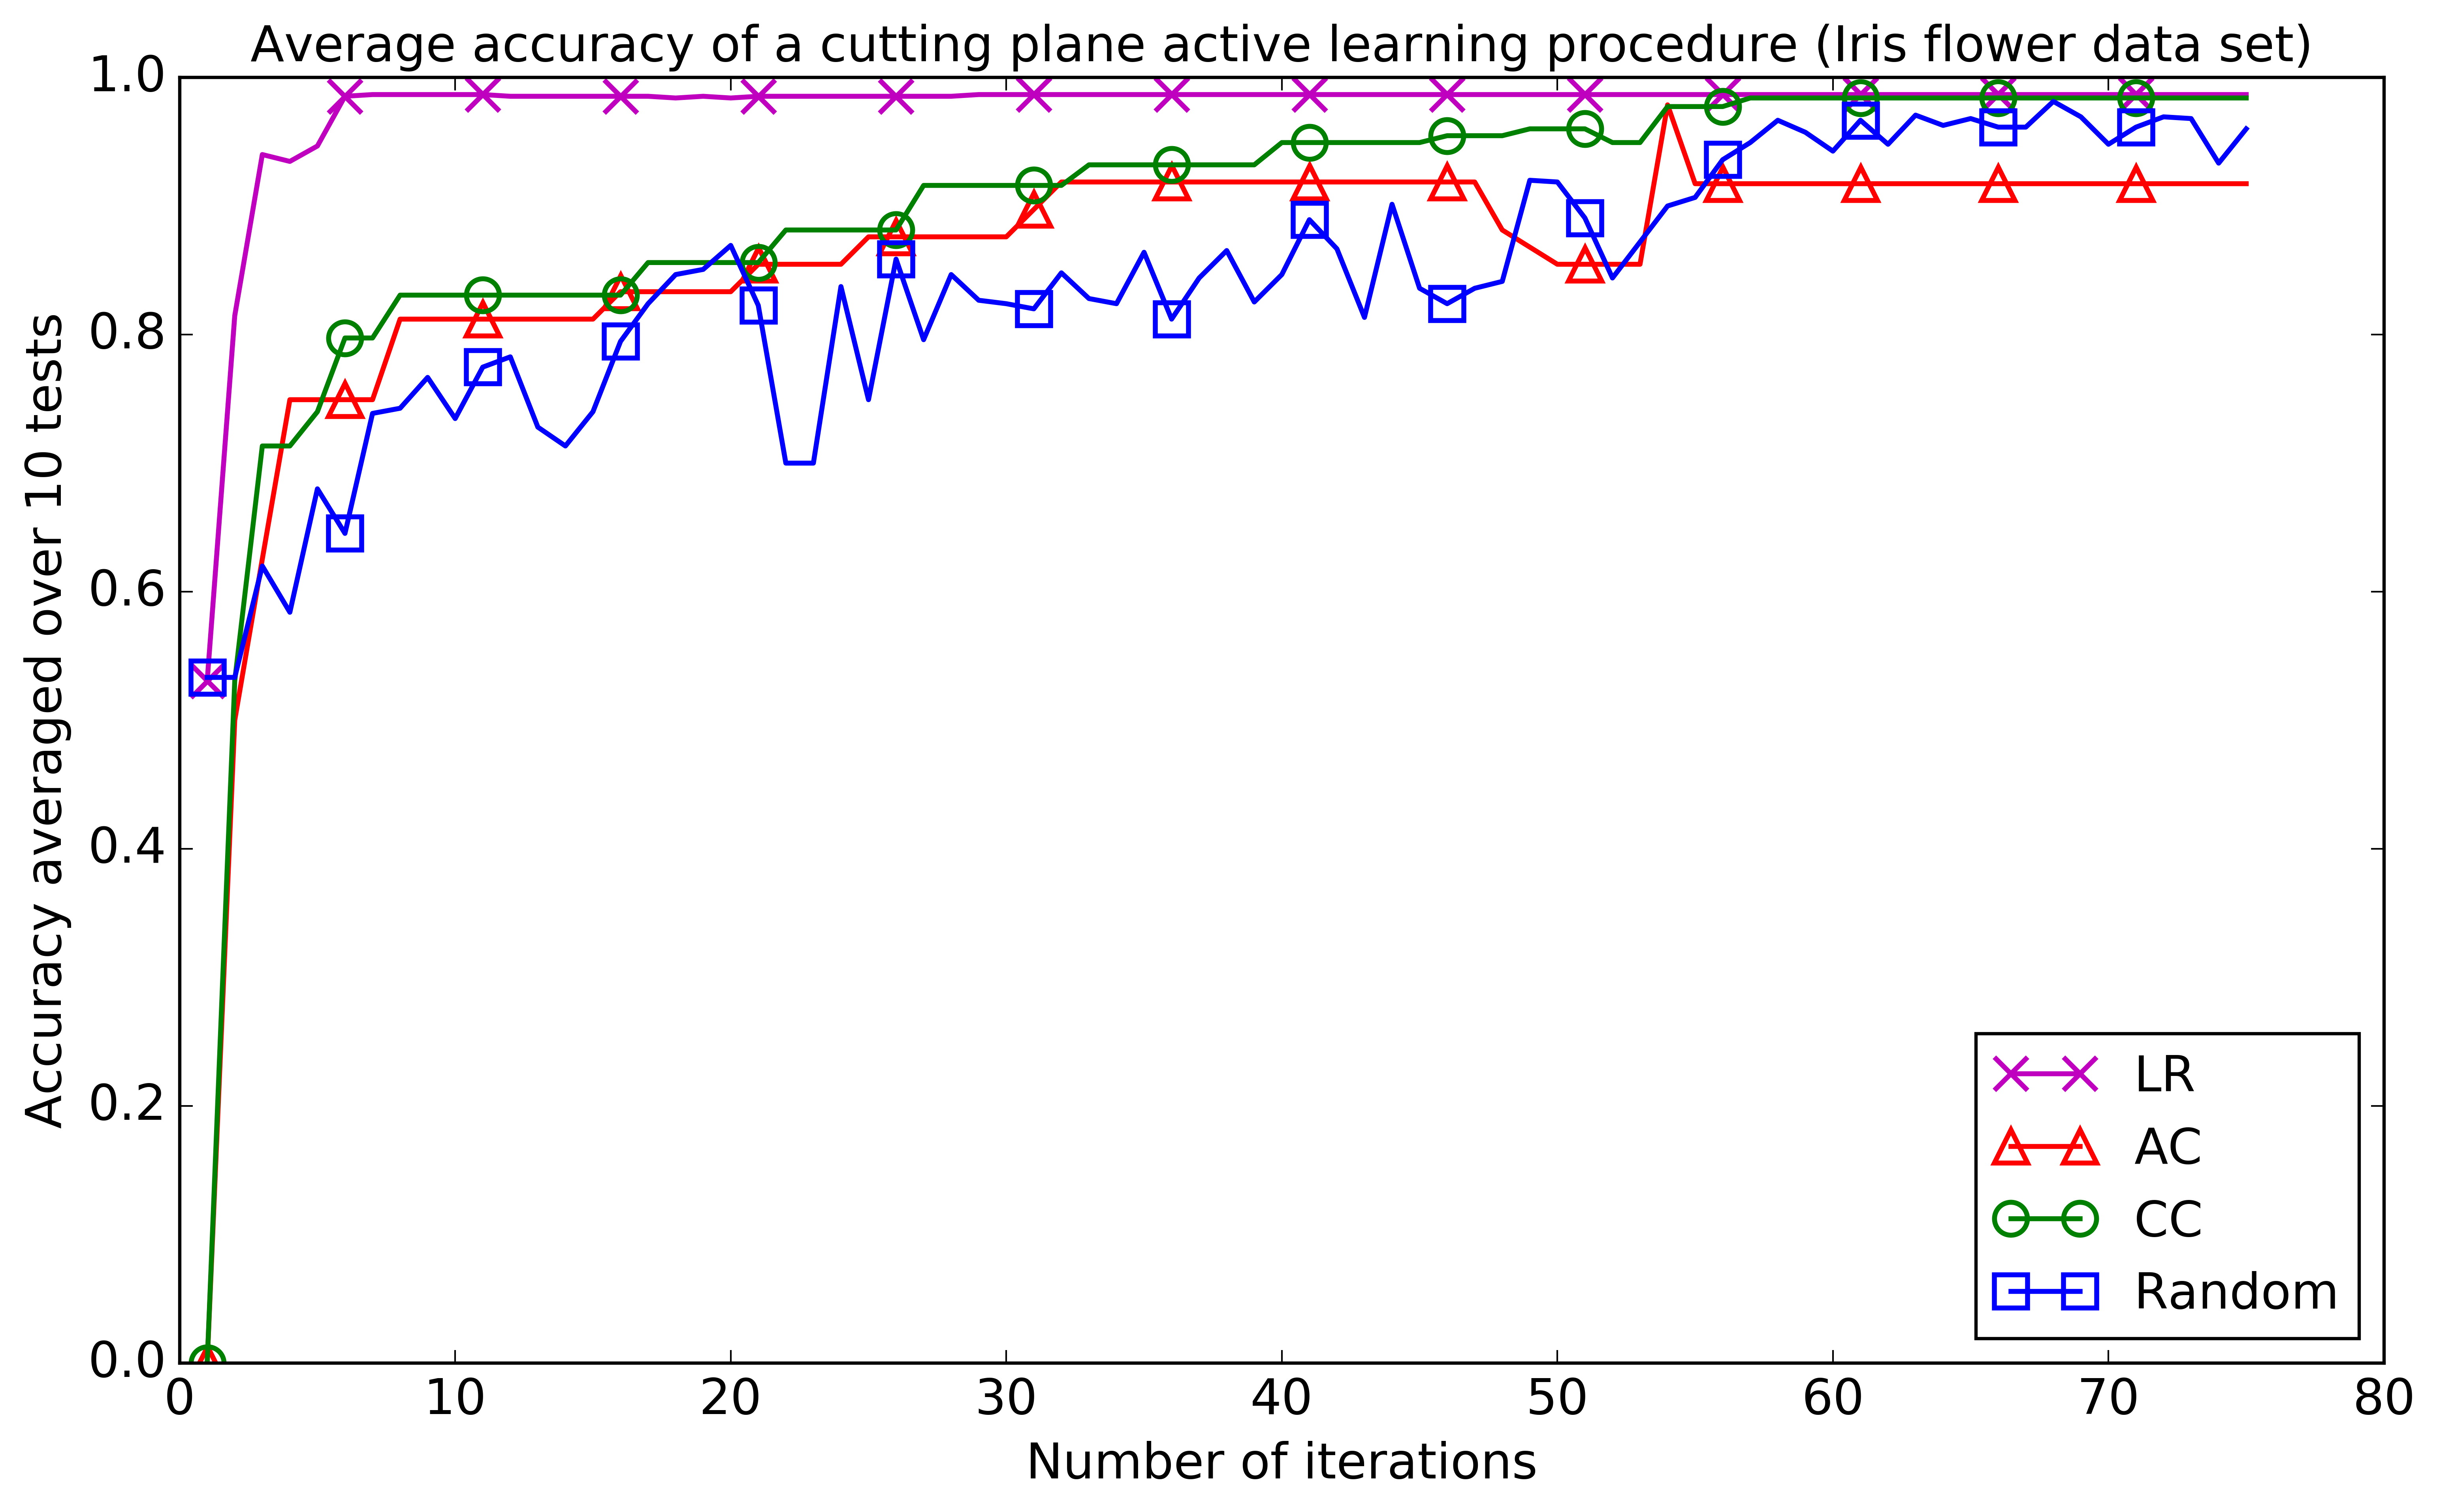
\includegraphics[width=\linewidth]{figures/iris_experiment.png}
        %     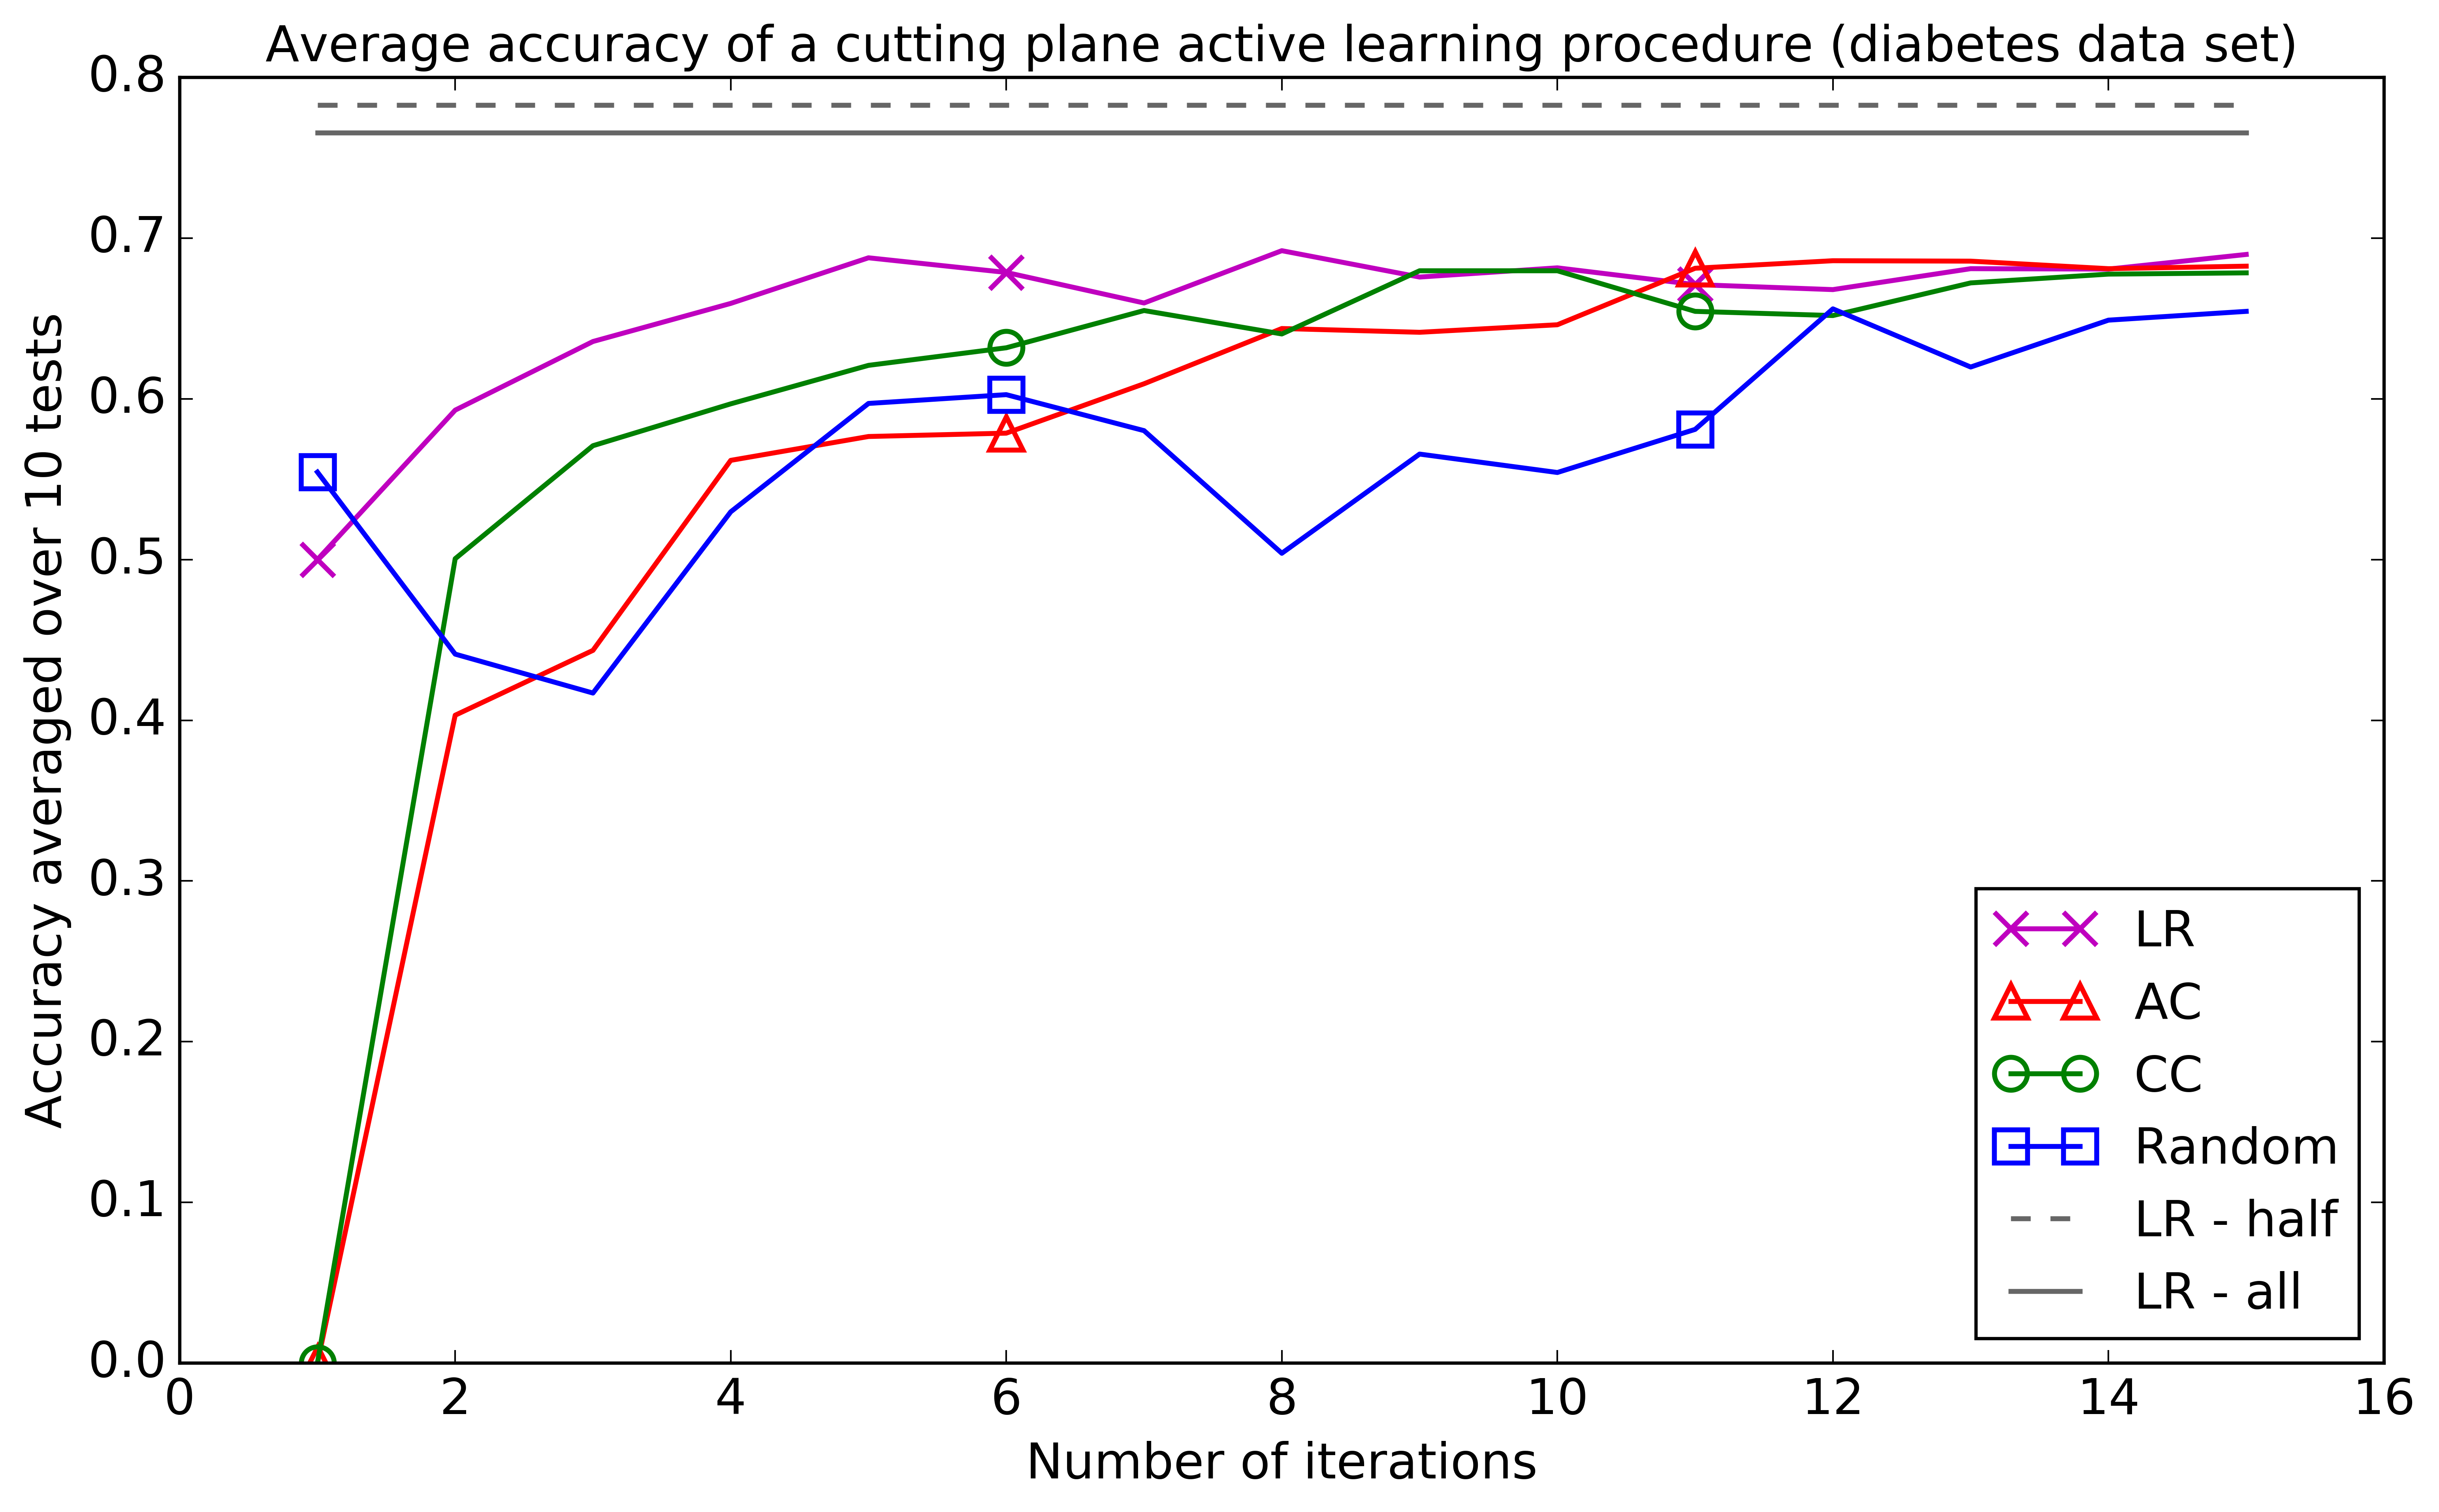
\includegraphics[width=\linewidth]{figures/diabetes_experiment.png}
        % \end{figure}
        % \newpage

    \subsection*{Discussion}
        In both the experiment on the Iris flower data set and the diabetes data set we see that our implementation of logistic regression (LR) trained on a random sample outperformed the active learning algorithm with query point as the AC (AC), CC (CC) and random center (Random). In Section \ref{s:conc} I will give suggestions on how the performance of the active learning algorithm could be improved.

        In the experiment with the Iris flower data set we see that overall CC outperformed AC and Random and performed on par with LR after approximately $55$ iterations. AC performed similarly to CC, and outperformed Random with the exception that after aproximately $45$ iterations the average accuracy of AC dropped signficantly. 

        Although I have not investigated this, it is possible that this can be attributed to a numerical computing error occuring once the candidate space $\mathcal{C}_k$ gets very small. This seems a reasonable suggestion given that the implementation of the AC computation is my own and numerical computing did arise during its development. Moreover, the smoother behavior of CC could be in part due to relying on the \texttt{scipy.optimize.linprog} function to compute the CC. 

        In the experiment with the diabetes data set we first observe that on average logistic regression trained on half the training data set (LR-- half) and the whole training data set (LR--all) performed the best but still with average accuracy less than 80\%. Indeed, it is interested to observe that LR--half ourperformed LR--all, which could possibly be attributed to the data set not being linearly seperable. Like the experiment on the Iris flower data set we see that AC and CC outperformed random and CC outperformed AC.

        LR signficantly outperformed AC and CC on the Iris flower data set and while it also outperformed AC and CC on the diabetes data set this was not as significantly and after roughly $9$ iterations, LR, AC and CC performed approximately equally. 

        In regards to the experiment on the diabetes data set, it is worth noting that I only included data up to labelling at most $15$ points as the computation time grew exponentially with the maximum number of points to be labelled. Having said this, there is partial date for labelling at most $30$ points, which took approxiately $36$ hours to compute. This running time growth be attributed to using rejection sampling to sample the points in the \textsc{Query} function. Specifically, random vectors were drawn from a nine-dimensional hypercube centered at the origin and were rejected if they did not lie in the current candidate space $\mathcal{C}_k$. We see this in how computing each of AC, CC and Random in the case of labelling at most $15$ points involved generating at least $1, 000, 000$ random vectors while the case of labeling at most $30$ points involved generating at least $1, 000, 000, 000$ random vectors.

\section{Conclusion and further directions}\label{s:conc}


\appendix

\section{The Cholesky factorization}\label{a:cholesky}

\section{Subgradients: basic definitions and results}\label{a:subgrad}

\section{Computing the analytic center analytically: sample calculations}\label{a:sample}

\section{The barrier method and basic phase I method}\label{a:barrier}


\renewcommand\refname{Bibliography}
\begin{thebibliography}{99}
    % \bibitem[Bis06]{bishop_06} C. Bishop. \emph{Pattern Recognition and Machine Learning}. Springer, 2006.
    % \bibitem[Boy08a]{Boy08} S. Boyd. \emph{Lecture 6 $|$ Convex Optimization II (Stanford)}. 2008. \url{https://youtu.be/N3vJOq5ZmKc}.
    % \bibitem[Boy08b]{Boy08b} S. Boyd. \emph{Lecture 7 $|$ Convex Optimization II (Stanford)}. 2008. \url{https://youtu.be/t0MmgkV4YrA}.
    \bibitem[BV04]{BV04} S. Boyd and L. Vandenberghe. \emph{Convex Optimization}. Cambridge University Press, 2004.
    \bibitem[BVS08]{BVS08} S. Boyd, L. Vandenberghe and J. Skaf. \emph{Analytic Center Cutting-Plane Method}. 2008. \url{https://see.stanford.edu/materials/lsocoee364b/06-accpm_notes.pdf}.
    \bibitem[BV11]{BV11} S. Boyd and L. Vandenberghe. \emph{Localization and Cutting-Plane Methods}. 2011. \url{http://web.stanford.edu/class/ee364b/lectures/localization_methods_notes.pdf}.
    \bibitem[BDV15]{BDV15} S. Boyd, J. Duchi and L. Vandenberghe. \emph{Subgradients}. 2015. \url{http://web.stanford.edu/class/ee364b/lectures/subgradients_notes.pdf}.
    \bibitem[Das11]{Das11} S. Dasgupta. (2011). Two faces of active learning. \emph{Theoretical Computer Science}, Volume 412, Issue 19, pp. 1767-1781.
    \bibitem[LR15]{LR15} U. Louche and L. Ralaivola. (2015). From Cutting Planes Algorithms to Compression Schemes and Active Learning. \emph{2015 International Joint Conference on Neural Networks}, pp. 1-8.  
\end{thebibliography}

% Examples:
% \bibitem[AHU]{ahu} Aho, A.,\ Hopcroft, J.,\ and Ullman, J.\ (1976). {\em{The Design and Analysis of Computer Algorithms.}} Addison Wesley, Reading, Mass.

% \bibitem[AT]{AT} Auslander, L. and Tolmieri, R. (1979). Is Computing with the Fast Fourier Transform Pure or Applied Mathematics? {\em{Bulletin (New Series) of the AMS Vol. 1}} 847-897.

% [Lee03] John Lee, \emph{Introduction to Topological Manifolds}, Springer Science, New York, USA, 2003.

% [Rat06] John Ratcliffe, \emph{Foundations of Hyperbolic Manifolds}, Springer Science, New York, USA, 2006.

\end{document}